% THIS IS AN EXAMPLE DOCUMENT FOR VLDB 2012
% based on ACM SIGPROC-SP.TEX VERSION 2.7
% Modified by  Gerald Weber <gerald@cs.auckland.ac.nz>
% Removed the requirement to include *bbl file in here. (AhmetSacan, Sep2012)
% Fixed the equation on page 3 to prevent line overflow. (AhmetSacan, Sep2012)

\documentclass{sig-alternate-05-2015}
\usepackage{graphicx}
\usepackage{balance}  % for  \balance command ON LAST PAGE  (only there!)
\usepackage{cleveref}
\usepackage{times}
\usepackage{url}

\newcommand\system{\textsc{SourceSight}}
\newtheorem{definition}{Definition}

\makeatletter
\makeatother

\begin{document}

% ****************** TITLE ****************************************
\CopyrightYear{2016} \setcopyright{acmcopyright}
\conferenceinfo{SIGMOD '16,}{June 26--July 1, 2016, San Francisco, CA, USA.}
\isbn{978-1-4503-3531-7/16/06}\acmPrice{\$15.00}
\doi{http://dx.doi.org/10.1145/2882903.2899403}

\clubpenalty=10000 
\widowpenalty = 10000

\title{{\LARGE \system}: Enabling Effective Source Selection}

\numberofauthors{3} 

\author{
% 1st. author
\alignauthor
Theodoros Rekatsinas\\
       \affaddr{Stanford University}\\
       \email{thodrek@cs.stanford.edu}
% 2nd. author
\alignauthor
Amol Deshpande\\
       \affaddr{University of Maryland}\\
       \email{amol@cs.umd.edu}
% 3rd. author
\alignauthor 
Xin Luna Dong\\
       \affaddr{Google Inc.}\\
       \email{lunadong@google.com}
\and  % use '\and' if you need 'another row' of author names
% 4th. author
\alignauthor 
Lise Getoor\\
       \affaddr{UC Santa Cruz}\\
       \email{getoor@soe.ucsc.edu}
% 5th. author
\alignauthor Divesh Srivastava\\
       \affaddr{AT\&T Labs-Research}\\
       \email{divesh@research.att.com}
}

\maketitle

\begin{abstract}
Recently there has been a rapid increase in the number of data sources and data services, such as cloud-based data markets and data portals, that facilitate the collection, publishing and trading of data. Data sources typically exhibit large heterogeneity in the type and quality of data they provide. Unfortunately, when the number of data sources is large, it is difficult for users to reason about the actual usefulness of sources for their applications and the trade-offs between the benefits and costs of acquiring and integrating sources. In this demonstration we present \system, a system that allows users to interactively explore a large number of heterogeneous data sources, and discover valuable sets of sources for diverse integration tasks. \system~uses a novel multi-level source quality index that enables effective source selection at different granularity levels, and introduces a collection of new techniques to discover and evaluate relevant sources for integration.
\end{abstract}


\section{Introduction}
\label{sec:intro}
Data integration remains among the most cost-intensive tasks in data management, because of the considerable computation and human-curation costs involved in the process~\cite{kruse2015estimating} and, often times, the monetary cost involved in acquiring data~\cite{balazinska:vldb11}. With a rapid increase in the number of data sources available for consumption, facilitated in part by the rise of data markets~\cite{balazinska:vldb11} and public dataset repositories~\cite{datahub}, an additional challenge faced by a user is to {\em identify} the sources that are truly valuable and appropriate for her application. This gives rise to the natural question of how can one discover {\em the most valuable sources} for integration, i.e., sources that maximize the user's benefit (i.e., the utility of the data in the final integration result) at the minimum cost. 

Several approaches have been proposed to help users reason about the value of integrating multiple sources: (i) {\em cost-oriented} techniques that focus on characterizing solely the cost of integration, and (ii) {\em value-oriented} techniques that reason about the trade-off between the benefit and cost of integration. Techniques from the first category reason about the effort required to perform schema-matching, data-cleaning and data-transformation when integrating multiple sources~\cite{kruse2015estimating}; however, these techniques do not estimate the actual benefit of integration~\cite{rekatsinas:2015}. Existing value-oriented techniques focus on the marginal benefit of integrating a new source~\cite{dong:vldb13,rekatsinas:2014}. Nevertheless, they typically assume that users have already identified {\em all} sources relevant to their application and do not allow users to explore and identify which sources are the most valuable for their desired {\em integration task}, nor do they support diverse integration tasks across multiple users.

To understand these limitations, consider companies, such as Dataminr, Bloomberg, Thomson-Reuters, etc., that integrate data streams from multiple news sources into unified real-time feeds for clients in finance, the public sector, news, security and crisis management. Each client-specific task is associated with a different {\em integration task}, i.e., multiple news sources are combined together to construct the necessary feeds. Moreover, client-tasks are diverse and can be characterized by a set of named entities, such as people, locations, or specific topics, such as finance or terrorism etc. Due to the large number of sources it is unlikely that users know in advance all sources that provide valuable data for their task. Thus, it is essential to allow multiple users to discover and select sources based purely based on their integration task description. 

Recent research has shown that carefully selecting data sources can dramatically improve the quality of integrated data both in terms of accuracy~\cite{dong:vldb13} and timeliness~\cite{rekatsinas:2014,rekatsinas:sdm15}. This can, in turn, improve the performance of intelligence applications, such as disease outbreak forecasting~\cite{rekatsinas:sdm15}, or demonstration and civil unrest monitoring~\cite{ramakrishnan2015model}, or can help businesses minimize the monetary cost of their integration pipelines by enabling them to detect and acquire only the most valuable sources for their applications~\cite{dong:vldb13}.

Motivated by the above, we recently introduced our vision for a {\em data source management system}~\cite{rekatsinas:2015} that enables users to discover the most valuable sources for their applications. In this demonstration proposal, we present \system, a fully functional prototype of such a data source management system. We also discuss extensions to our initial design that allow a user to evaluate the effectiveness of the system (\Cref{sec:extensions}) at selecting sources automatically. The core of the system is built around {\em source selection}~\cite{dong:vldb13} allowing one to reason about the trade-offs between the benefit and cost of integration. The benefit of integration can be quantified using a variety of metrics, such as coverage, accuracy, timeliness and bias~\cite{rekatsinas:2015}. The cost of integration is quantified using a model similar to that of Dong et al.~\cite{dong:vldb13}; other cost models~\cite{kruse2015estimating} can be seamlessly incorporated in our system. \system~offers a number of unique features:

\vspace{2pt}\noindent (1) Users can describe the domain of their integration task using a keyword-based interface and explore sources as well as similar integration tasks relevant to their task.

\vspace{2pt}\noindent (2) Given an integration task, users can perform source selection using a variety of quality metrics. \system~casts source selection as a multivariate optimization problem to help users understand the actual trade-offs between different quality metrics and proposes different sets of sources to be used when different weights are assigned to different quality metrics. 

\vspace{2pt}\noindent (3) Finally, the system allows users to interactively edit the recommended solutions by adding or deleting sources. Users can also perform a qualitative comparison between different sets of sources. This is crucial for evaluating the solutions recommended by \system~and aids the users to understand why a particular set of sources was proposed by the system.

\noindent\textbf{Related work.} Over the past few years, the research community has introduced a number of techniques to support search over large numbers of datasets in the form of Web tables~\cite{limaye:2010,dassarma:2012}. Unlike \system, these techniques focus on providing rankings of datasets and are agnostic to the cost or benefit of integrating multiple datasets. Apart from Web table search, more generic data search systems, such as Microsoft's Power BI\footnote{http://www.microsoft.com/en-us/powerbi}, have been recently proposed. Nonetheless, while facilitating data integration, they do not help analysts to understand the quality of data sources.

\section{Discovering Valuable Sources}
\label{sec:sources}
Consider a user who wants to find sources relevant to an integration task, e.g., a data scientist exploring datasets in a repository such as DataHub~\cite{datahub} or a journalist compiling information from multiple news sources in a repository such as EventRegistry\footnote{http://eventregistry.org/}. While users can provide a keyword-based description of their task, they may not know all the relevant sources. Our goal is twofold: 

\begin{figure}
	\begin{center}
	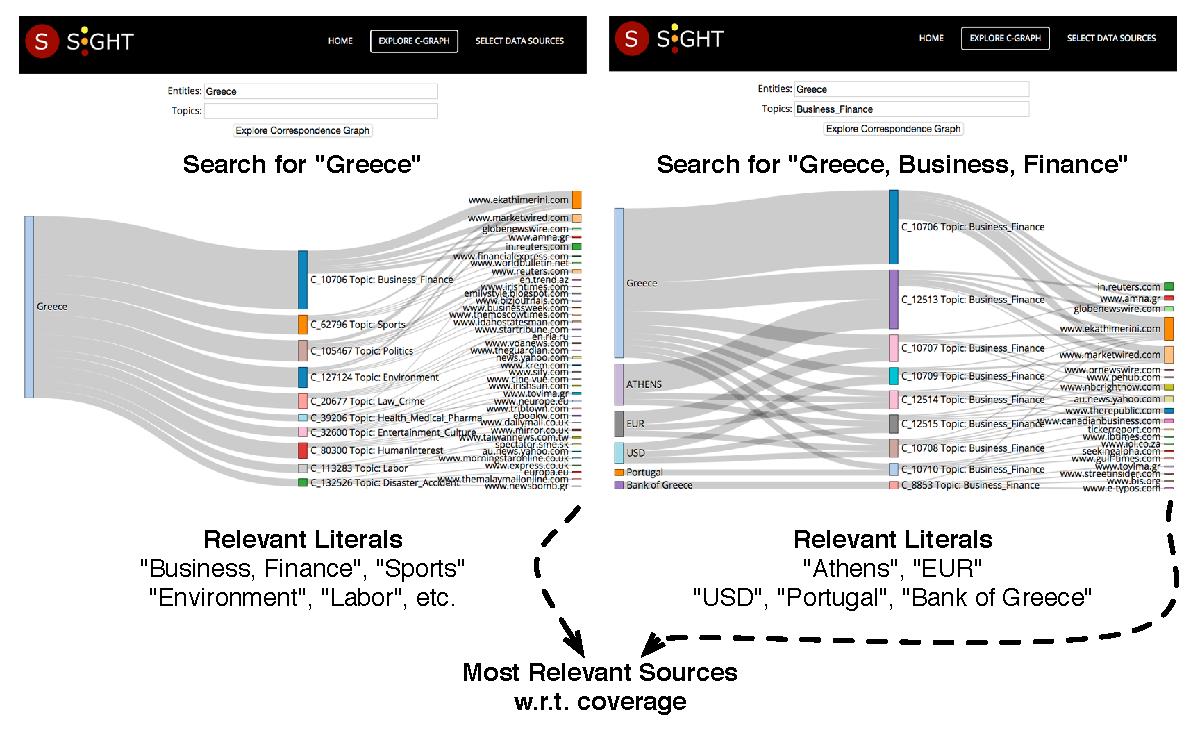
\includegraphics[trim=0 0 0 60, clip,width=0.50\textwidth]{fig/exploreCor}
	\vspace{-20pt}
	\caption{Discovering relevant sources and refining an integration task with \system.}
	\label{fig:exploration}
	\end{center}
	\vspace{-25pt}
\end{figure}


First, users should be able to provide a keyword-based description of their task and {\em discover} sources relevant to it. Further, it would be beneficial to explore related and more specialized task descriptions as the set of relevant sources may change significantly. \system~is the first system that unifies these two aspects of source exploration into a common interface. \Cref{fig:exploration} shows an example use-case where a journalist wants to write an overview article about the socio-economic situation in Greece. The journalist starts by requesting news sources relevant to the keyword ``Greece''. Apart from presenting the relevant sources, \system~additionally recommends that it might be beneficial to explore related and more specialized descriptions, such as ``Greece and Business and Finance'' or ``Greece and Labor'', as the set of relevant sources may change significantly. Based on these recommendations the user can revise her integration task description and obtain a new more focused set of relevant sources.

Second, sources discovered in the previous step may exhibit large heterogeneity. They may provide stale or erroneous data~\cite{Dong_vldb:2009, li:2012}, they may contain duplicate data~\cite{bronzi:2013, li:2012} at different costs, and may exhibit schema or instance heterogeneity. Given this diversity in the sources, the users need to be able to reason about the utility of integrating together a {\em set} of sources; a user should be able to find a set of sources that satisfy any cost constraints that she has, and if integrated together will maximize the {\em benefit} of integration. 

To support this, \system~allows users to perform {\em source selection}~\cite{dong:vldb13}, i.e., choose a subset of sources among a set of relevant sources $S$ identified using keyword search and exploration. Let $B(\bar{S},I)$ denote the benefit of integrating sources $\bar{S}$ with respect to an integration task $I$, and let $C(\bar{S})$ denote the total integration cost for $\bar{S}$. Source selection finds a set of sources $S_I$ such that $S_I = \arg\max_{\bar{S} \subseteq S}B(\bar{S},I) - C(\bar{S})$. To quantify the benefit of integration, \system~uses a range of rigorous data quality metrics, such as {\em coverage}, {\em accuracy}, {\em timeliness} and {\em bias}~\cite{rekatsinas:2015}. 

\begin{figure}
	\begin{center}
	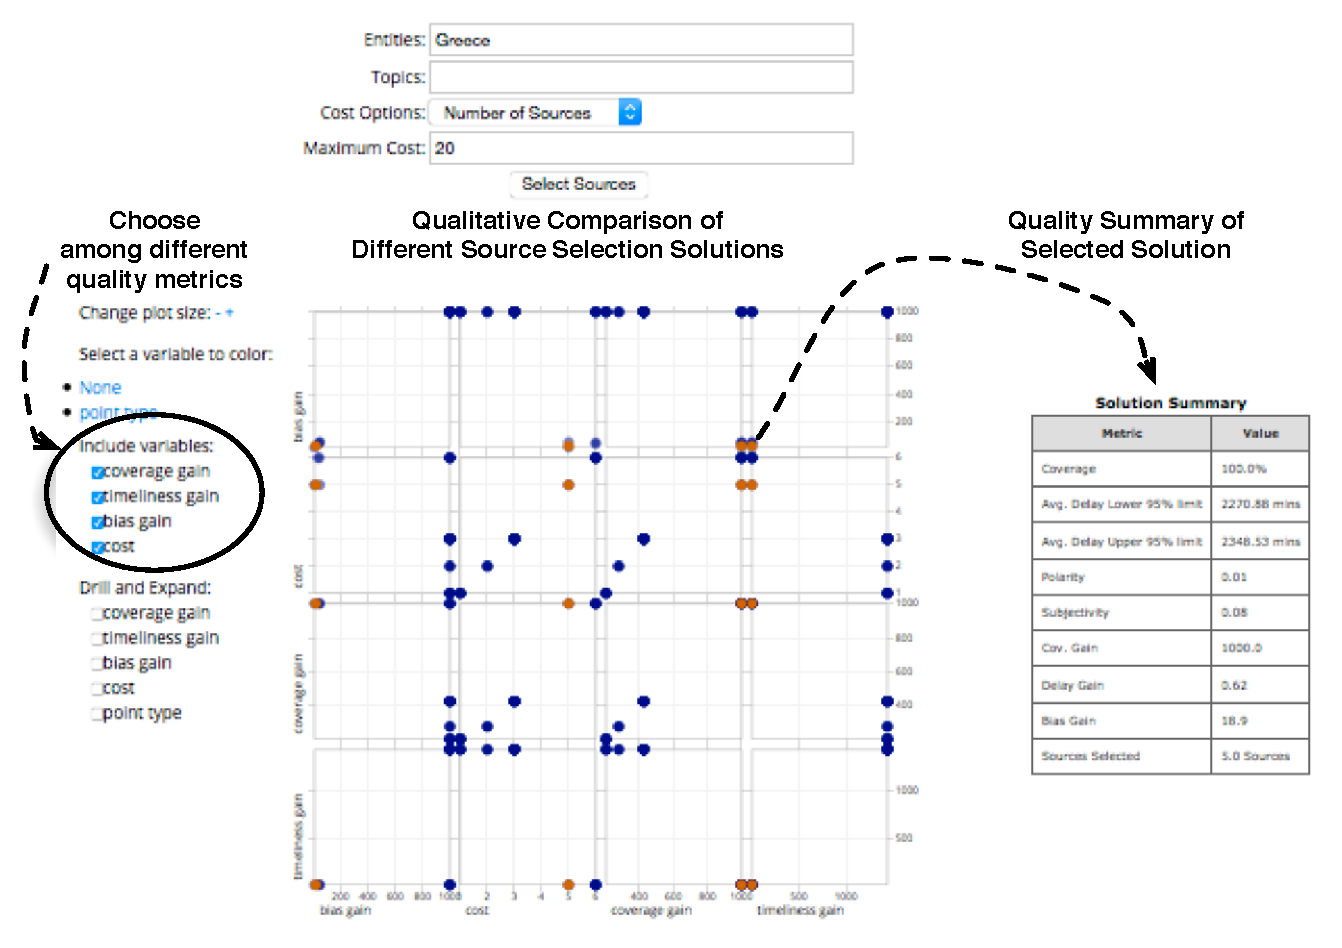
\includegraphics[trim=0 0 0 85, clip,width=0.40\textwidth]{fig/ssResults}
	\vspace{-10pt}
	\caption{\system's interface for exploring different source selection solutions.}
	\label{fig:ssresults}
	\end{center}
	\vspace{-22pt}
\end{figure}

Given this variety of quality metrics, \system~provides the user with multiple source selection solutions that correspond to different weighting configurations for the available quality metrics. This allows users to explore different trade-offs amongst the available quality metrics and identify the set of sources that best satisfies their quality requirements (see \Cref{fig:ssresults}).

\section{{\Large \system} Design}
\label{sec:design}
Recently, we put forward our vision about the functionalities and architecture of data source management systems for effective source selection~\cite{rekatsinas:2015}. 
\system~is a realization of such a system. Next, we present \system's architecture, how it implements (Sections~\ref{sec:integtask} and \ref{sec:sourcesel}) the functionalities described in~\cite{rekatsinas:2015}, and new functionalities (\Cref{sec:extensions}) \system~provides.

\begin{figure}[h]
    \centering
    	\vspace{-5pt}
    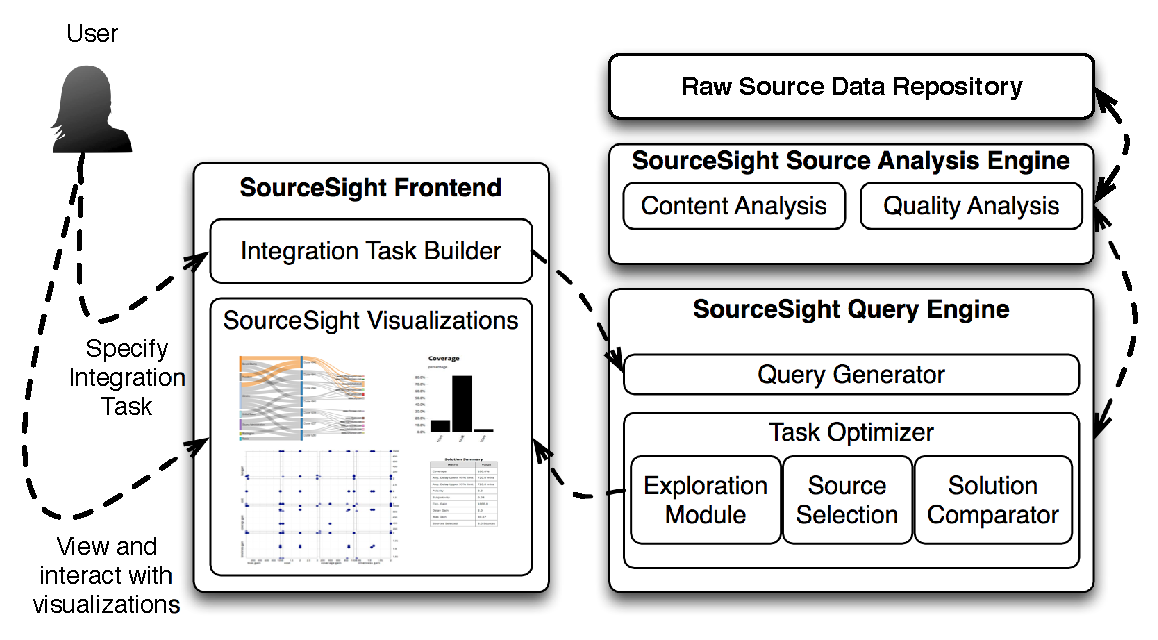
\includegraphics[width=0.4\textwidth]{fig/srcsightOver}
    	\vspace{-10pt}
    \caption{\system~architecture.}
    \label{fig:architecture}
    	\vspace{-15pt}
\end{figure}

\subsection{Architecture overview}
\system~is built as a layer on top of a data source repository that stores the raw data of data sources. Acquisition of the data sources is out of the scope of this work. The system consists of three components: a front-end, a source analysis engine and an exploration engine (\Cref{fig:architecture}). 
The basic operations of \system~can be divided into an {\em offline} phase and an {\em online} phase. In the offline phase, the source analysis module constructs an index describing both the content and the quality of each source with respect to multiple quality metrics. This index is used during the online phase to serve user requests. We discuss the indexing technique in more detail in \Cref{sec:reasoning}. In the online phase, users interact with \system~via its front-end module and user requests are served by the exploration engine. Users can specify a desired integration task by providing a keyword-based description of their integration task. Once a description is provided, users can choose among three main functionalities: They can (i) choose to explore which keywords and sources are most relevant to their task, (ii) choose to perform source selection, or (iii) choose to perform a qualitative comparison between different sets of sources constructed either manually or automatically via source selection. 

\subsection{Reasoning about the content of sources}
\label{sec:reasoning}
We assume that each entry in a source (e.g., a tuple in a table or a news article in a news media source) is associated with a set of {\em context literals} and all context literals come from a {\em literal dictionary} $V$. We assume that $V$ is hierarchically structured and edges between literals can encode containment, equivalence and other semantic relations. For example, $V$ can be a knowledge base with literals corresponding to {\em real-world entities} and {\em concepts}. \Cref{fig:kgcg} shows an example knowledge base with concept literals being hierarchically structured (e.g., ``Country'' is subsumed by ``Location'') and entity literals being semantically associated with concept literals (e.g., ``USA'' has a specific ``Population''). Dictionary $V$ allows us to identify the domains covered by each source by analyzing the union of context-literal sets for the entries of the source. 

\begin{figure}[h]
	\begin{center}
	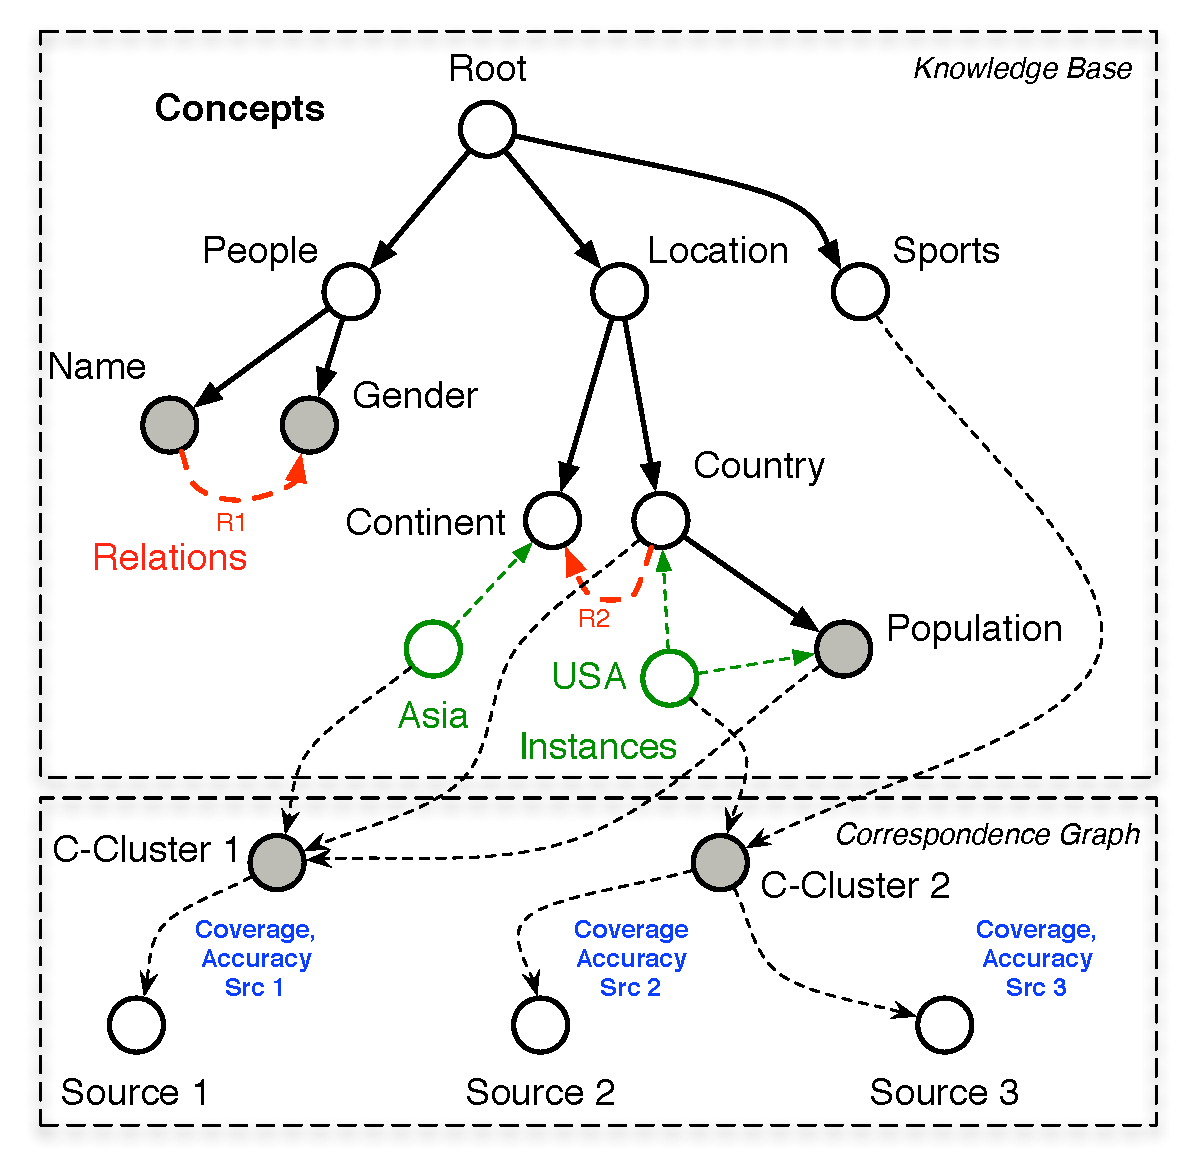
\includegraphics[clip,scale=0.25]{fig/kgcg}
	\vspace{-10pt}
	\caption{An example knowledge base with the corresponding correspondence graph.}
	\label{fig:kgcg}
	\vspace{-15pt}
	\end{center}
\end{figure}

To reason about the content and quality of different sources we augment $V$ with a {\em correspondence graph}~\cite{rekatsinas:2015}. An example of a correspondence graph is shown in \Cref{fig:kgcg}. The nodes in the correspondence graph are either data sources ({\em source nodes}) or clusters of literals as dictated by the available sources ({\em c-cluster nodes}). The edges in the correspondence graph connect each source node with c-cluster nodes and c-cluster nodes with the corresponding literals in the knowledge base.  In the example above, there are two c-cluster nodes, one corresponding to the population of countries in Asia and one to sports in the USA (i.e., ``USA and Sports''). The edges connecting c-cluster nodes to literals follow conjunctive semantics. Each edge from a source to a c-cluster node is annotated with a quality profile of that source for that specific c-cluster, and each c-cluster node is associated with local information about the dependencies of the data sources that are connected to it. 

The correspondence graph serves as a content and quality index for the available sources. To construct it we first learn the latent c-cluster nodes and then compute the quality profiles and data source dependencies for each c-cluster node. To discover the literals associated with each source entry we use Thomson Reuters' Open Calais\footnote{http://www.opencalais.com/}, an API for semantic annotations with respect to multiple knowledge bases including DBpedia, Freebase and others. To construct the c-cluster nodes we adopt a frequent pattern mining approach based on the FP-growth algorithm~\cite{Han:2000}. This allows discovering domains that are prevalent in multiple sources. After discovering the c-cluster nodes, we compute the quality of each source with respect to each c-cluster node it is connected to. To do this, we collectively analyze the content of all sources connected to a c-cluster node to form a single dataset characterizing the content of the c-cluster and then each individual source is compared with the combined data to compute its quality~\cite{rekatsinas:2015}. 

\subsection{Specifying an integration task}
\label{sec:integtask}
\system~allows users to specify an integration task $I = (I_d, I_c)$ by providing a description that corresponds to a context-literal set $I_d$ defining the {\em domain} of the task and potentially a set of integration cost constraints $I_c$. The system recommends literals and sources that are related to their keyword search, enabling them to either explore sources relevant to their search or refine their initial task description by considering related literals.

Relevant context-literals are all literals that are related to literals in $I_d$ either via $V$ or via the correspondence graph. The former accounts for semantic relations across literals while the second accounts for co-occurrence of literals in a source. Similarly, relevant sources to task $I$ are all data sources that provide entries whose context-literal set is a subset of $I_d$ or related to $I_d$ via the literal dictionary $V$ (e.g., using equivalence or containment relationships). 

\system~offers a unified interface for users to explore both context-literals and sources related to their desired integration task (see \Cref{fig:exploration}). Given an integration task description $I_d$, \system~returns the set of top relevant literals to the search of the user as well as the most relevant sources with respect to coverage or other metrics for the specified keyword search. The user can then select any of the recommended sources to view a summary of the literals that the source covers as well as a quality summary of the source for the corresponding keyword search. Users can also choose to update their integration task description $I_d$ by including new relevant context-literals to $I_d$.

\subsection{Multivariate source selection}
\label{sec:sourcesel}
Given an integration task $I = (I_d,I_c)$, the user can perform source selection with respect to the context-literals $I_d$ and the constraints $I_c$. As discussed in \Cref{sec:sources}, \system~considers multiple quality metrics to quantify the benefit of integration. The system casts source selection as a multi-objective optimization problem and finds the set of {\em Pareto optimal} solutions corresponding to the source selection problem at hand. 

Discovering all the solutions on the Pareto front is expensive as one needs to reason about all the potential trade-offs amongst the available quality metrics. To address this issue we use a sampling strategy to discover solutions that correspond to different quality trade-offs. Let $Q$ be the set of quality metrics under consideration and $B_q(\cdot)$ be an oracle computing the benefit of integration with respect to quality metric $q \in Q$ for any set of sources. We compute the total benefit of integration as a weighted linear combination of the individual benefit of each quality metric, i.e., $B(\cdot) = \sum_{q \in Q} w_q \cdot B_q(\cdot)$. Given this definition of the total benefit of integration, we sample different combinations of the weights $w_q$ and solve source selection for each of those. Finally, we identify the Pareto optimal solutions amongst the sampled solutions. 

The sampled solutions are presented to the user in a way that makes it easy to compare the quality of each solution. The corresponding interface is shown in \Cref{fig:ssresults}. Users can select a particular solution and view a concise summary of the benefit and cost of integration achieved by it. Users can also drill down and expand only on a subset of the available quality metrics to fully understand specific trade-offs across different solutions. Finally, users can view a detailed description of a source selection solution with information about the sources included in the result and their individual contributions to the quality of the final integration result. 

\subsection{Comparing sets of sources}
\label{sec:extensions}
\system~enables users to understand why a particular set of sources was recommended to them and evaluate its performance. Users can perform a qualitative comparison between two sets of sources with respect to the same integration task (\Cref{fig:comparison}). They are also able to examine how two sets of sources compare against each other with respect to individual quality metrics, as well as the total integration benefit and cost. The sets of sources to be compared can correspond to recommended solutions from source selection or can be manually constructed by the user as follows: (i) users can start from a returned source selection solution and add new sources or remove already included sources, or (ii) users can manually select individual sources and construct their own set. The former allows them to examine the neighborhood of the returned solution but also serves as a mechanism of convincing the user of the value achieved by the output of source selection. To enable the latter, \system~provides users with the top-$k$ most relevant sources for their integration task with respect to each individual quality metric.
\begin{figure}
	\begin{center}
	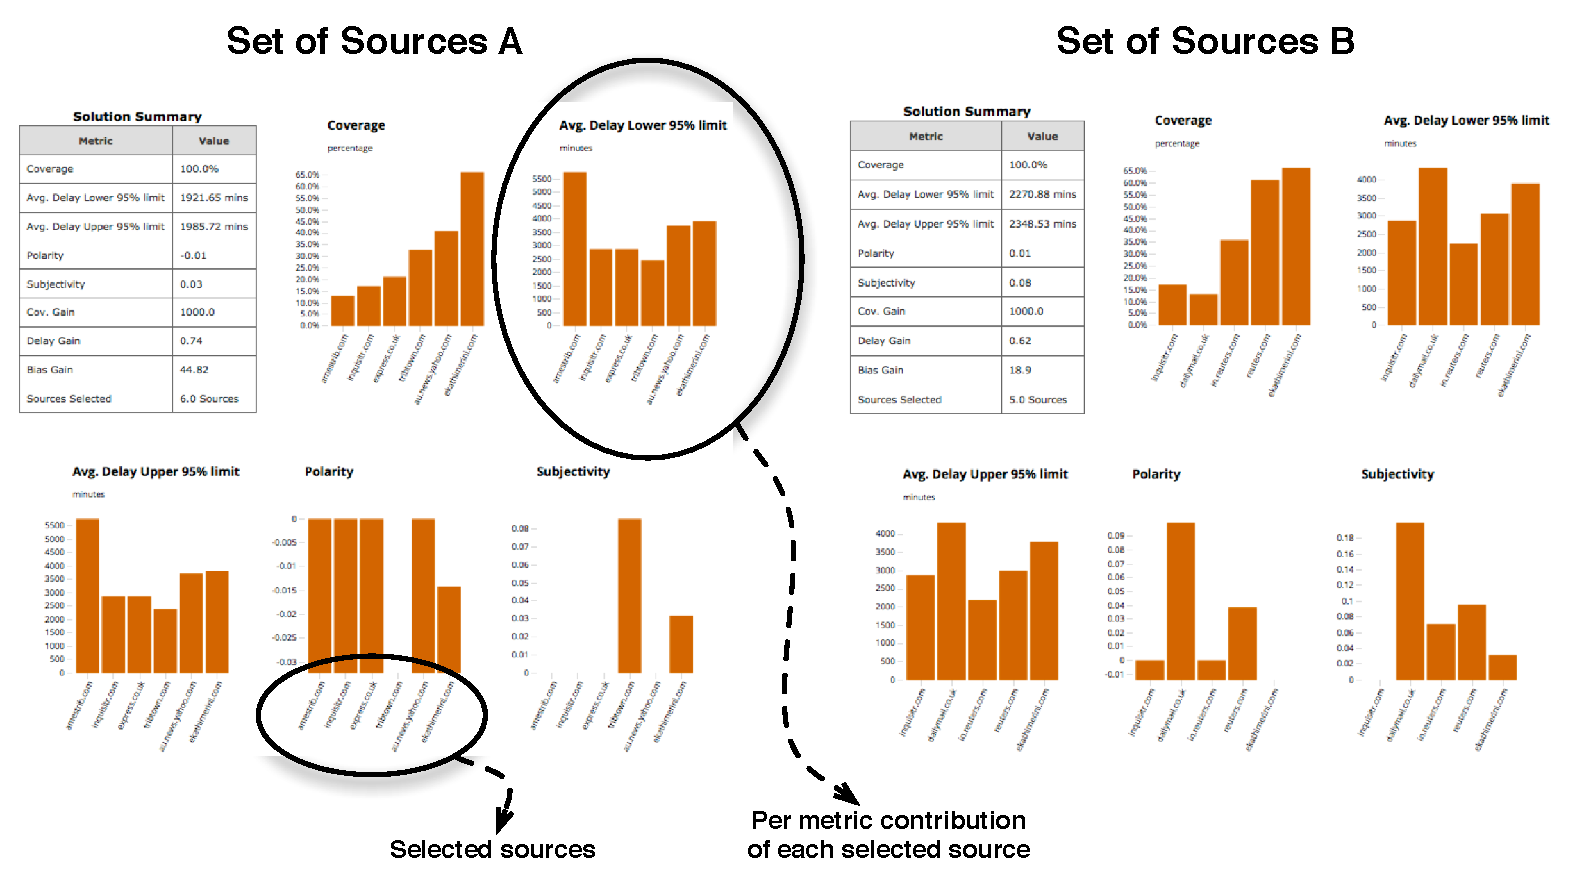
\includegraphics[trim=0 0 0 0, clip,width=0.5\textwidth]{fig/compSS}
	\vspace{-20pt}
	\caption{Comparing sets of sources.}
	\label{fig:comparison}
	\vspace{-25pt}
	\end{center}
\end{figure}

\vspace{-5pt}
\section{Demo Details}
\label{sec:details}
We will demonstrate the functionality of \system~through hands-on experience with two real-world scenarios. With the data stored on a remote server, users will interact with the system via a web interface. Our goals are two fold: (i) demonstrate the utility of \system~in exploring and selecting beneficial sources for integration, and (ii) demonstrate the effectiveness of automatic source selection for diverse integration tasks. 

\vspace{2pt}\noindent\textbf{Scenarios.} The first scenario corresponds to that of identifying the most valuable news data sources providing events for different locations, people, etc. The underlying data consists of event extractions collected from EventRegistry, a repository that monitors news media from all over the world. The dataset contains 15,000 data sources which correspond to news domains and quality metrics such as coverage, timeliness or position bias of the articles that are inherently relevant. EventRegistry gets updated at fixed intervals by ingesting feeds of newly extracted news articles. EventRegistry is the right fit to demonstrate the usefulness and practicality of \system~due to the large number of data sources available, the available updates over time, and the heterogeneity that the sources exhibit both with respect to their domains and their quality. We plan to use a recent snapshot retrieved from EventRegistry containing at least six months of news article data. 

The second scenario corresponds to that of enriching an existing genomics knowledge base recording the interactions between genes and phenotypes. Constructing knowledge bases by analyzing vast amounts of scientific literature is gaining more and more traction in several domains~\cite{Niu_deepdive:web-scale}. However, a critical pain point in those applications is identifying the most relevant scientific articles to analyze and extract information from so that the coverage and accuracy of the knowledge base is improved. To demonstrate this scenario we will use the abstracts of scientific articles collected by PubMed and we will consider expanding a knowledge base constructed by DeepDive\footnote{http://deepdive.stanford.edu/}. The total number of articles is 359,324 and each article corresponds to a data source. The goal of this scenario is to demonstrate how users can use source selection techniques to identify the most valuable sources that will improve the quality and expand a running integrated dataset.


\vspace{2pt}\noindent\textbf{Demonstrating Utility.} Attendees will be able to describe ad-hoc tasks or use pre-formulated integration tasks in \system. Then they will have the opportunity to evaluate the source exploration and source selection functionalities offered by \system. Our goal is for users to understand the trade-offs between different quality metrics of sources in both datasets we have described above and understand how \system~can guide them to select the most suitable set of sources for their application needs.

\vspace{2pt}\noindent\textbf{Demonstrating Effectiveness.} For this part of the demo users will mainly interact with the third functionality of \system, i.e., comparing and contrasting sets of sources. Attendees will compare sets of sources provided by source selection with manually created sets of sources and understand the quality differences across them. 

{\scriptsize
\begin{thebibliography}{10}
%\bibitem{powerbi}
%Excel Power BI.
%\newblock \url{http://www.microsoft.com/en-us/powerbi}.

\bibitem{balazinska:vldb11}
M.~Balazinska, B.~Howe, and D.~Suciu.
\newblock Data markets in the cloud: An opportunity for the database community.
\newblock {\em PVLDB}, 2011.

\bibitem{datahub}
A.~Bhardwaj, S.~Bhattacherjee, A.~Chavan, A.~Deshpande, A.~J. Elmore,
  S.~Madden, and A.~G. Parameswaran.
\newblock Datahub: Collaborative data science \& dataset version management at
  scale.
\newblock In {\em CIDR}, 2015.

\bibitem{bronzi:2013}
M.~Bronzi, V.~Crescenzi, P.~Merialdo, and P.~Papotti.
\newblock Extraction and integration of partially overlapping web sources.
\newblock {\em PVLDB}, 2013.

\bibitem{dassarma:2012}
A.~Das~Sarma, L.~Fang, N.~Gupta, A.~Halevy, H.~Lee, F.~Wu, R.~Xin, and C.~Yu.
\newblock Finding related tables.
\newblock In {\em SIGMOD}, 2012.

\bibitem{Dong_vldb:2009}
X.~L. Dong, A.~Halevy, and C.~Yu.
\newblock Data integration with uncertainty.
\newblock {\em VLDB Journal}, 2009.

\bibitem{dong:vldb13}
X.~L. Dong, B.~Saha, and D.~Srivastava.
\newblock Less is more: selecting sources wisely for integration.
\newblock {\em PVLDB}, 2012.

\bibitem{Han:2000}
J.~Han, J.~Pei, and Y.~Yin.
\newblock Mining frequent patterns without candidate generation.
\newblock In {\em SIGMOD}, 2000.

\bibitem{kruse2015estimating}
S.~Kruse, P.~Papotti, and F.~Naumann.
\newblock Estimating data integration and cleaning effort.
\newblock In {\em EDBT}, 2015.

\bibitem{li:2012}
X.~Li, X.~L. Dong, K.~Lyons, W.~Meng, and D.~Srivastava.
\newblock Truth finding on the deep web: is the problem solved?
\newblock {\em PVLDB}, 2013.

\bibitem{limaye:2010}
G.~Limaye, S.~Sarawagi, and S.~Chakrabarti.
\newblock Annotating and searching web tables using entities, types and
  relationships.
\newblock {\em PVLDB}, 2010.

\bibitem{Niu_deepdive:web-scale}
F.~Niu, C.~Zhang, C.~R\'e, and J.~Shavlik.
\newblock Deepdive: Web-scale knowledge-base construction using statistical
  learning and inference.
\newblock In {\em VLDS}, 2012.

\bibitem{ramakrishnan2015model}
N.~Ramakrishnan, C.~Lu, M.~Marathe, A.~Marathe, A.~Vullikanti, S.~Eubank,
  S.~Leman, M.~Roan, J.~Brownstein, K.~Summers, et~al.
\newblock Model-based forecasting of significant societal events.
\newblock {\em Intelligent Systems, IEEE}, 30:86--90, 2015.

\bibitem{rekatsinas:2014}
T.~Rekatsinas, X.~L. Dong, and D.~Srivastava.
\newblock Characterizing and selecting fresh data sources.
\newblock In {\em SIGMOD}, 2014.

\bibitem{rekatsinas:2015}
T.~Rekatsinas, X.~L. Dong, L.~Getoor, and D.~Srivastava.
\newblock {Finding Quality in Quantity: The Challenge of Discovering Valuable
  Sources for Integration}.
\newblock In {\em CIDR}, 2015.

\bibitem{rekatsinas:sdm15}
T.~Rekatsinas, S.~Ghosh, S.~Mekaru, E.~Nsoesie, J.~Brownstein, L.~Getoor, and
  N.~Ramakrishnan.
\newblock Sourceseer: Forecasting rare disease outbreaks using multiple data
  sources.
\newblock In {\em SDM}, 2015.

\end{thebibliography}}

%{\scriptsize 
%\bibliographystyle{abbrv}
%\bibliography{srcsight}}

\end{document}
